\chapter{Establishing a Baseline}
\label{ch:baseline}

This chapter establishes a robust MLP actor baseline for the IEEE 14-bus task.

\section{Evaluation Protocol}
\label{sec:results-evaluation-protocol}

All experiments use an 80/20 train/test chronic split. The 80\% training split is used for policy updates, while the 20\% test split estimates generalization. Evaluation rollouts run periodically during training using 10 episodes per split. 
\\
\\
The primary performance metric is test episodic survival (expressed as a percentage), representing the fraction of evaluation timestep where the agent survives and successfully prevents a blackout. Results are reported using seed-aggregated mean curves, with shaded regions indicating variability. Final evaluations report the performance of the checkpoint that achieved the highest training survival.

\section{IEEE 14-Bus Experiments}
\label{sec:bus14-results}

The initial MAPPO baseline from the MARL2Grid framework lead to unstable policies and low survival rates on the IEEE 14-bus topology-control task. The following experiments test training and architectural modifications to establish a high-performing baseline.

\subsection{MLP Baseline}
\label{subsec:a0-core-reruns}

\paragraph{Question.}
Which changes are needed to obtain a stable MLP MAPPO baseline on the 14-bus
task?

\paragraph{Baseline and changes.}
We start from the MLP MAPPO baseline of the MARL2Grid framework and test several main
stabilization choices:

\begin{itemize}
  \item using reward normalization;
  \item changing the critic update so that the critic is updated once for the
  whole batch instead of once per agent;
  \item tuning of optimization hyperparameters to stabilize the training, as summarized in Table~\ref{tab:new-hyperparameters}.
\end{itemize}

\begin{table}[H]
  \centering
  \small
  \caption{New hyperparameters for MAPPO training.}
  \label{tab:new-hyperparameters}
  \begin{tabular}{lrr}
    \toprule
    Hyperparameter & New Value & Paper Baseline \\
    \midrule
    \textbf{ENVIRONMENT} & & \\
    n\_envs (number parallel environment) & 20 & 10 \\
    \midrule
    \textbf{PPO OPTIMIZATION} & & \\
    Total time step & 15,000,000 & 25,000,000 \\
    Actor learning rate & 1e-4 & 3e-5 \\
    Critic learning rate & 1e-4 & 3e-5 \\
    Gamma & 0.9 & 0.99 \\
    Update epochs & 10 & 80 \\
    Minibatches & 16 & 4 \\
    Maximum gradient norm & 1.0 & 10.0 \\
    \bottomrule
  \end{tabular}
\end{table}

\paragraph{Evidence.}
Table~\ref{tab:a0-core-summary} reports final and peak survival for the core
ablations. Figure~\ref{fig:rerun-a0-all} overlays all
core MLP baseline curves.

\paragraph{Interpretation.}
The \texttt{Optimized MLP Baseline}, which combines reward normalization and an optimized critic update, achieves the best performance and convergence speed, yielding the highest and most stable final survival (\(\sim\)93\%). Removing or reducing any of these three elements, using a smaller architecture, disabling reward normalization, or reverting to a non-optimized critic update, results in a drop in either learning speed or final survival. The original unoptimized baseline fails entirely to learn a competitive policy. Because the \texttt{Optimized MLP Baseline} consistently outperforms the ablations, it is established as the standard reference for all subsequent comparisons.

\begin{table}[H]
  \centering
  \scriptsize
  \caption{MLP baseline run configurations. The reference run is
  \texttt{Optimized MLP Baseline}.}
  \label{tab:a0-run-configurations}
  \setlength{\tabcolsep}{3pt}
  \begin{tabular}{L{0.25\textwidth}L{0.13\textwidth}L{0.09\textwidth}L{0.11\textwidth}L{0.11\textwidth}L{0.20\textwidth}}
    \toprule
    Run family & Actor/critic hidden layers & Reward norm. & Initial action-0 prob. &
    Optimized critic update & Difference from \texttt{Optimized MLP Baseline} \\
    \midrule
    \texttt{Optimized MLP Baseline} & \(3\times256\) / \(3\times256\) &
    true & 0.0 & true & Reference baseline \\
    \texttt{Disable optimized critic update} & \(3\times256\) / \(3\times256\) &
    true & 0.0 & false & Disables optimized critic updates \\
    \texttt{Smaller MLP actor/critic} & \(2\times256\) / \(2\times256\) &
    true & 0.0 & true & Uses a smaller MLP actor and critic \\
    \texttt{Disable reward normalization} & \(3\times256\) / \(3\times256\) &
    false & 0.0 & true & Disables reward normalization \\
    \texttt{Old baseline (no val)} & \(3\times256\) / \(3\times256\) &
    true & 0.3 & false & Uses action-0 bias 0.3 and non-optimized critic updates \\
    \texttt{Initial Bias 50\%} & \(3\times256\) / \(3\times256\) &
    true & 0.5 & true & Uses action-0 bias 0.5 \\
    \texttt{Initial Bias 70\%} & \(3\times256\) / \(3\times256\) &
    true & 0.7 & true & Uses action-0 bias 0.7 \\
    \bottomrule
  \end{tabular}
\end{table}

\begin{figure}[H]
  \centering
  
\includegraphics[width=\textwidth]{figures/rerun_a0_core_all_curves.png}
  \caption{All MLP baseline core rerun survival curves shown on one axis.}
  \label{fig:rerun-a0-all}
\end{figure}

% \begin{figure}[H]
%   \centering
%   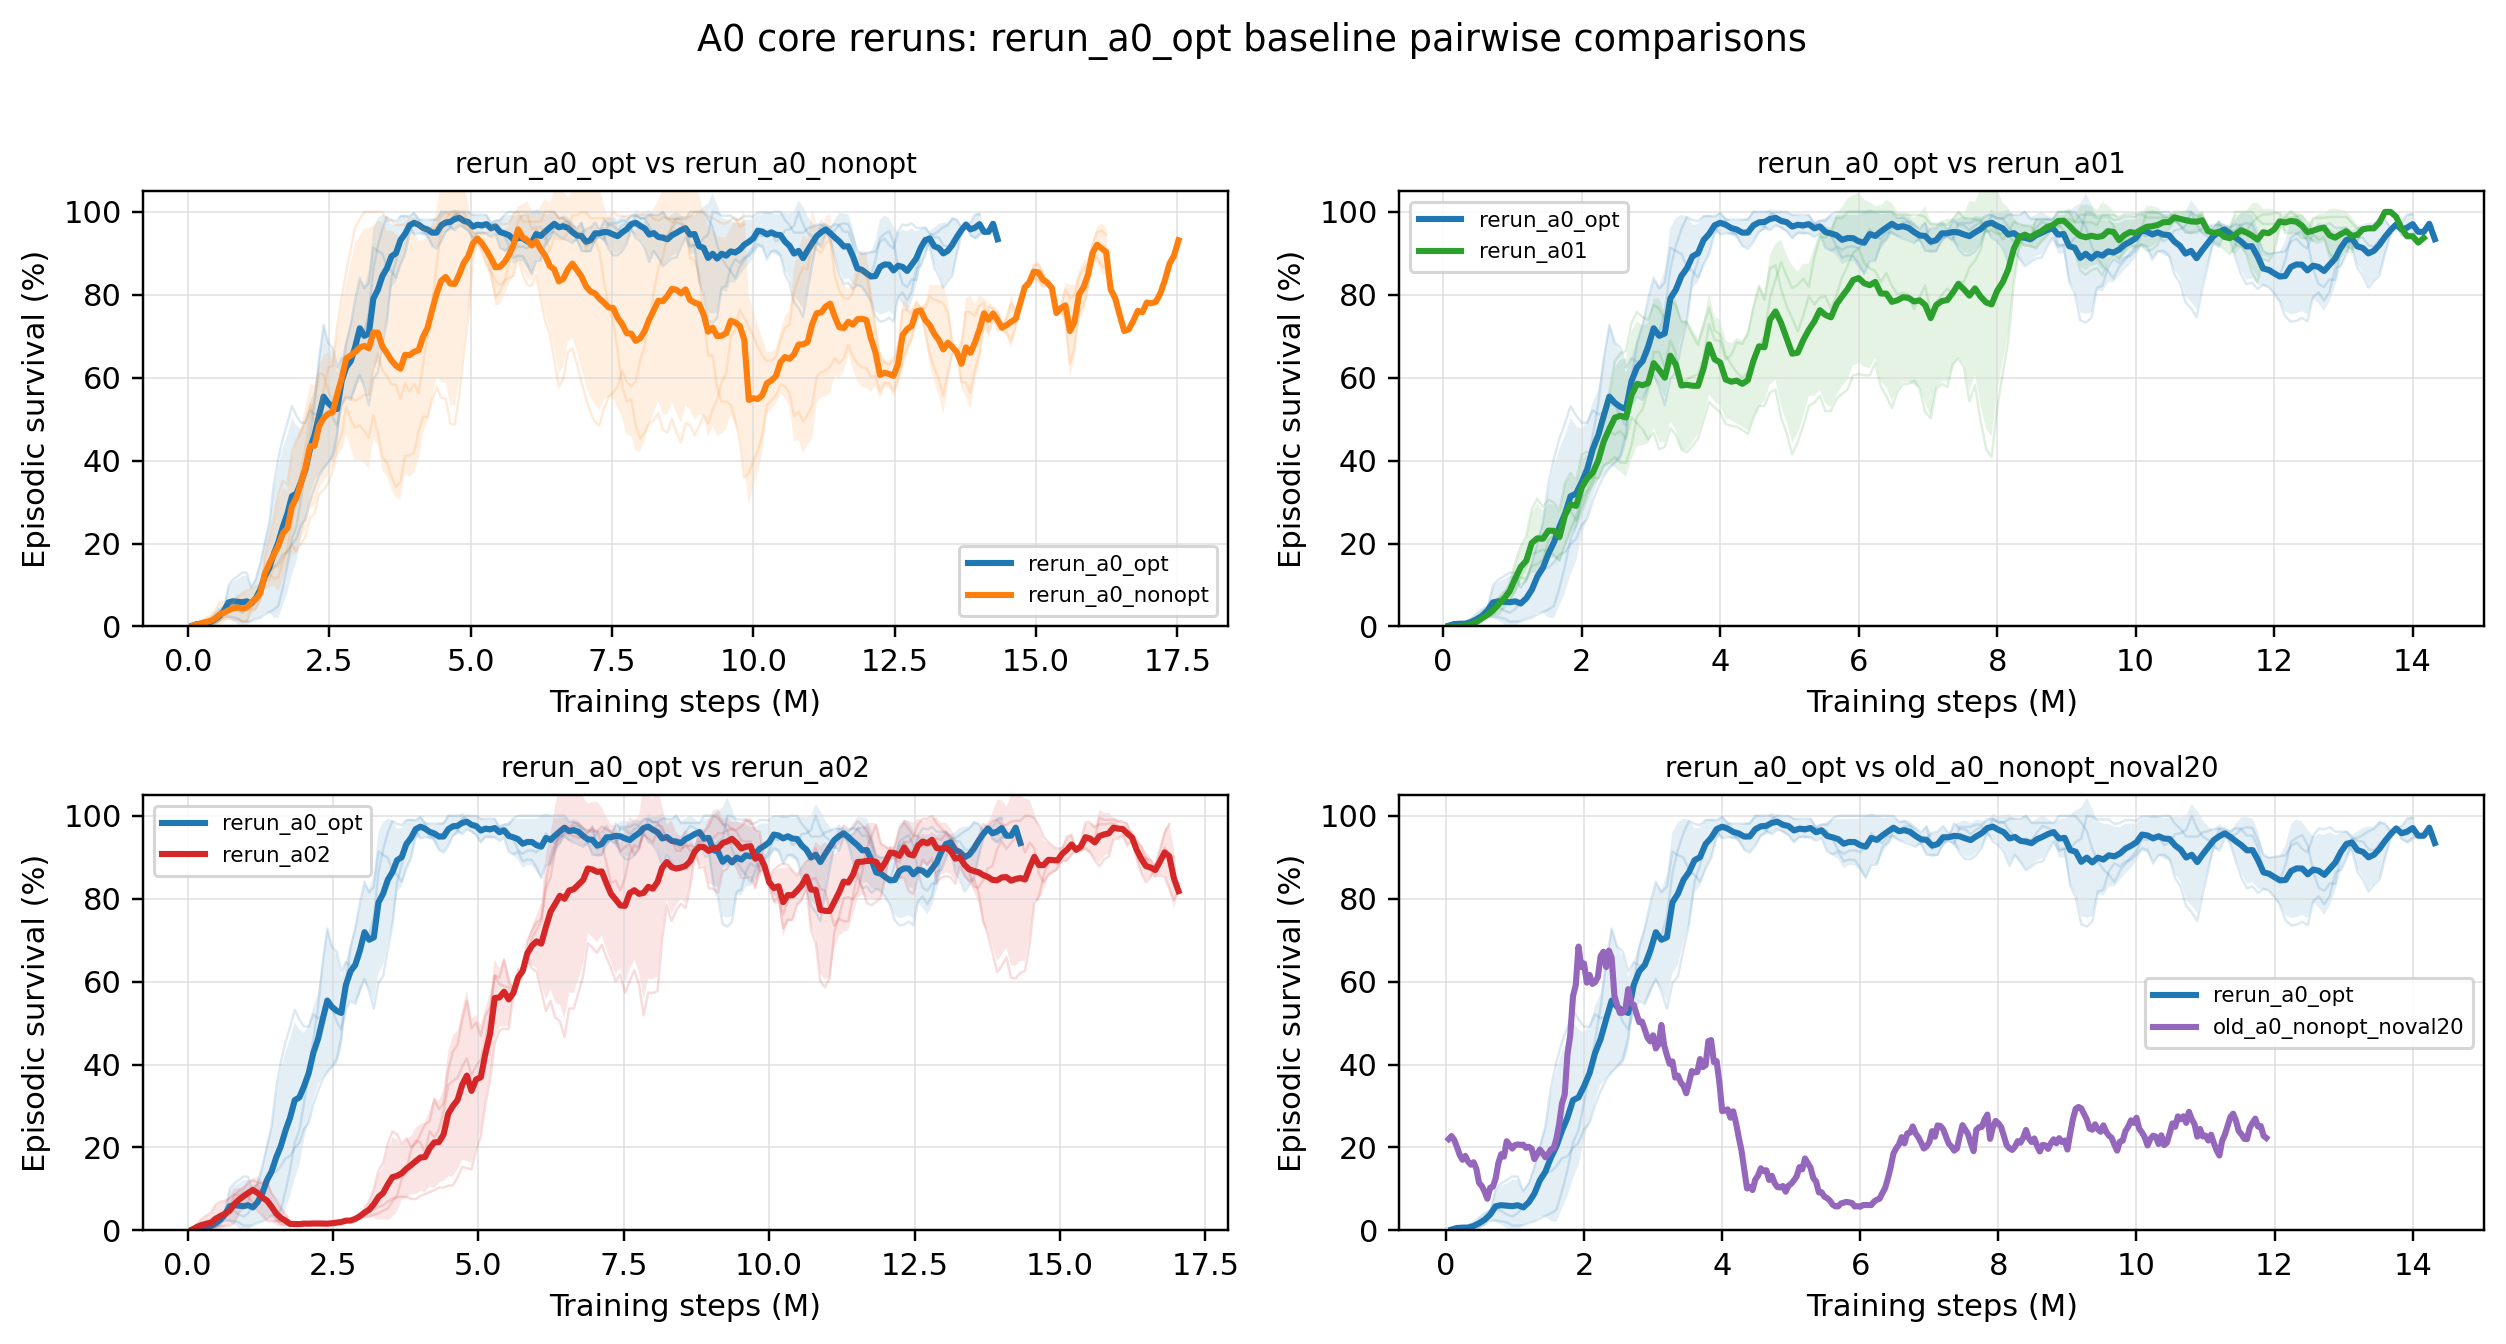
\includegraphics[width=\textwidth]{figures/rerun_a0_core_pairwise_comparisons.png}
%   \caption{Pairwise MLP baseline rerun comparisons against the \texttt{Optimized MLP Baseline}.}
%   \label{fig:rerun-a0-pairwise}
% \end{figure}

\begin{table}[H]
  \centering
  \small
  \caption{MLP baseline core rerun survival summary.}
  \label{tab:a0-core-summary}
  \resizebox{\textwidth}{!}{%
  \begin{tabular}{llrr}
    \toprule
    Run & Intended change & Final survival (\%) & Peak survival (\%) \\
    \midrule
    \texttt{Optimized MLP Baseline} & Optimized MLP baseline & 93.4 & 98.6 \\
    \texttt{Disable optimized critic update} & Non-optimized critic update & 93.1 & 95.8 \\
    \texttt{Smaller MLP actor/critic} & Smaller MLP architecture & 93.7 & 100.0 \\
    \texttt{Disable reward normalization} & No reward normalization & 81.8 & 97.1 \\
    \bottomrule
  \end{tabular}
  }
\end{table}

\subsection{Initial Do-Nothing Bias}
\label{subsec:a0-bias-reruns}

\paragraph{Question.}
Does biasing the initial policy toward action 0, the do-nothing action, help or
hurt learning? In theory, a do-nothing bias makes sense because in reality, human operators most often do not operate the grid (i.e., they take no action) under normal conditions.

\paragraph{Baseline and changes.}
Our baseline uses no initial do-nothing bias in this rerun set. The bias
controls keep the same general protocol but change the initial probability mass
assigned to action 0.


\paragraph{Implementation detail.}
The bias is applied only at initialization: it changes the starting action
distribution before learning, without changing the reward, architecture, or PPO
objective. This is implemented by artificially increasing the initial pre-softmax logits for the do-nothing action, such that the policy initially selects this safe action with a higher probability before any learning updates occur. This makes the ablation a test of exploration bias rather than a test
of representational capacity.

\paragraph{Evidence.}
Table~\ref{tab:a0-bias-summary} and Figure~\ref{fig:rerun-a0-bias} compare the
zero-bias baseline with \texttt{Initial Bias 50\%} and
\texttt{Initial Bias 70\%}.

\paragraph{Interpretation.}
The effect of the action-0 bias is large and non-monotonic. The 0.5-bias curve
remains unstable and substantially below the zero-bias baseline, whereas the
0.7-bias curve eventually reaches the highest final survival in this comparison.
The current conclusion is that adding an initialization bias is generally hurtful or highly unstable for the models. Instead of aiding exploration, a strong initialization prior appears to restrict the agent's ability to reliably discover diverse beneficial actions and should be treated cautiously as a first-order ablation variable.

\begin{table}[H]
  \centering
  \small
  \caption{Initial do-nothing bias survival summary.}
  \label{tab:a0-bias-summary}
  \begin{tabular}{lrr}
    \toprule
    Run & Final survival (\%) & Peak survival (\%) \\
    \midrule
    \texttt{Optimized MLP Baseline} & 93.4 & 98.6 \\
    \texttt{Initial Bias 50\%} & 50.8 & 70.2 \\
    \texttt{Initial Bias 70\%} & 99.3 & 100.0 \\
    \bottomrule
  \end{tabular}
\end{table}

\begin{figure}[H]
  \centering
  
\includegraphics[width=\textwidth]{figures/rerun_a0_bias_comparison.png}
  \caption{Optimized MLP baseline compared with initial do-nothing bias controls
  \texttt{Initial Bias 50\%} and \texttt{Initial Bias 70\%}.}
  \label{fig:rerun-a0-bias}
\end{figure}

\begin{tcolorbox}[colframe=red!75!black, colback=red!5!white, title=Chapter Summary]
\textbf{Objective:} Establish a stable, high-performing flat MAPPO baseline.
\\
\\
\textbf{Findings:}
\begin{itemize}
    \item \textbf{MLP optimization:} Hyperparameter tuning, reward normalization,
    and optimized critic updates raise the flat MLP baseline to roughly 93\%
    survival.
    \item \textbf{Do-nothing initialization:} The effect is large but
    non-monotonic; it is not a reliable substitute for learning when to
    intervene.
\end{itemize}
\vspace{0.35cm}
\textbf{Conclusion:} The tuned flat actor is a strong survival baseline. The
next step is to ask whether it can behave more like an operator by intervening
less often without losing that survival, which is the subject of
Chapter~\ref{ch:sparse-control}.
\end{tcolorbox}
